	% !TeX encoding = UTF-8
% !TeX spellcheck = pt_BR

%Intro começa aqui

\chapter{O futuro: cripto}

\begin{flushright}
	\begin{minipage}{8cm}
		\textit{	\noindent 
			\begin{flushright}
				``O que me afetou mais profundamente foi a percepção de que as ciências da criptografia e da matemática são ciências puras muito elegantes. Descobri que os fins para os quais essas ciências puras são usadas são menos elegantes.'' - Jim Sanborn (tradução livre)
		\end{flushright}}
		\vspace{1cm} 
	\end{minipage}
	\footnote{Citação original do inglês: ``What affected me most profoundly was the realization that the sciences of cryptography and mathematics are very elegant pure sciences. I found that the ends for which these pure sciences are used are less elegant.'' em entrevista com Milena Kalinovska \cite{SANBORN}}.
\end{flushright}

Neste capítulo mostraremos sobre o dinheiro do futuro, os criptoativos, relatando sua concepção e uma visão geral  sobre este tema. Mas antes faremos uma revisão rápida sobre criptografia.
  
 \section{Uma noção rápida sobre criptografia}
 \subsection{Idéia geral}
  
  A criptografia \index{Criptografia!Criptografia} pode ter várias definições \footnote{Segundo o dicionário Oxford \cite{OXDIC}, criptografia nada mais é que a arte de escrever ou resolver códigos.}\footnote{Conforme definido por \cite{RIVEST}, criptografia é a prática e o estudo de técnicas para comunicação segura na presença de comportamento adverso}. Como podemos notar observando estas definições, o início da história da criptografia data-se a medida que seres humanos iniciaram organizar em tribos, no qual já havia a necessidade de se comunicar, uma consequência disto seria a necessidade da comunicação em segredo. Na criptografia moderna\index{Criptografia!Criptografia Moderna}, não há somente a preocupação na resolução de problemas provenientes de ataques internos ou externos, mas também na melhoria da segurança digital sobre dados, informações, transações e computações distribuídas\footnote{Pode-se entender computação\index{Computação distribuída} distribuída como um sistema de processamento distribuído, ou seja, um sistema possuinte de múltiplos nós de processamento, porém interligados como um único sistema computacional. Veja \cite{PROG2} para saber mais}. Mais especificamente também são estudados autenticação de mensagens, assinaturas digitais, protocolos para troca de chaves secretas, protocolos de autenticação, dinheiro digital, leilões eletrônicos e eleições.  Até o final do século XX, a criptografia era considerada uma forma de arte, somente depois desse período ela começou a ser estudada de forma mais formal, com o desenvolvimento de uma teoria, sendo considerada assim uma ciência.
  
  
  A criptografia possui quatro objetivos:
  \begin{table}[H]
  \centering
  \begin{tabular}{|c|p{12cm}|}
  	\hline
  	\multicolumn{2}{|c|}{}\\
  	\multicolumn{2}{|c|}{Objetivos da criptografia} \\
  	\multicolumn{2}{|c|}{}\\
  	\hline
  	&\\
  	Confidencialidade & Somente o destinatário autorizado deve ser capaz de extrair o conteúdo da mensagem da sua forma cifrada. \\
  	&\\
  	\hline
  	&\\
  	Integridade & O destinatário deverá ser capaz de verificar se a mensagem foi alterada durante a transmissão. \\
  	&\\
  	\hline
  	&\\
  	Autenticação & O destinatário deverá ser capaz de verificar que se o remetente é realmente quem diz ser. \\
  	&\\
  	\hline
  	&\\
  	Irretratabilidade & Não deverá ser possível ao remetente negar a autoria de sua mensagem. \\
  	&\\
  	\hline
  \end{tabular}
\caption{Objetivos gerais da criptografia}
\end{table}
  
  \subsection{Métodos criptográficos históricos}
  
  Se considerarmos uma criptografia pré-computacional,  existem basicamente dois métodos para esconder as informações de uma mensagem. São eles a transposição e a substituição dos caracteres. Tais execuções poderiam então ser operadas pelo emissor e pelo destinatário da mensagem.
  \begin{itemize}\index{Tranposição (Criptografia)} \index{Substituição (Criptografia)}
  	\item No método da transposição, os conteúdos da mensagem criptografada e da mensagem original são idênticas, o que muda são a disposição das letras da mensagem.
  	\item No método por substituição cada letra permanece em seu devido lugar, porem ocorre uma substituição de acordo com uma tabela de referência que podem conter também figuras e símbolos.
  \end{itemize}

A cifra de César\index{Cifra de César}, que no caso trabalha com um valor fixo de saltos nas posições das letras do alfabeto é um exemplo clássico de criptografia por chave de substituição. O formato de medalhão pode ser facilmente adquirido atualmente conforme figura abaixo:

\begin{figure}[H]
	\centering
	\caption{Medalhão de cifra de César disponível para venda}
	\includegraphics[width=0.4\linewidth]{caesar_cipher.jpg}\\
	\text{Fonte: \cite{CAESAR}}
		
\end{figure}


  \subsection{Chaves criptográficas}
  Como pode-se notar, um algoritmo matemático fica responsável pelo segredo\footnote{Tal algoritmo criptografa a mensagem do remente e descriptografa ao chegar no destinatário} da chave criptográfica e é o segredo fundamental da criptografia. Existem dois tipos de chaves, conforme tabela:
  
  \begin{table}[H] \index{Chaves criptográficas!Chave simétrica} \index{Chaves criptográficas!Chave Assimétrica}
  	\begin{tabular}{|l|p{10cm}|}
  		\hline
  		\multicolumn{2}{|c|}{}\\
  		\multicolumn{2}{|c|}{Tipos de chaves criptográficas} \\
  		\multicolumn{2}{|c|}{}\\
  		\hline
  		&\\
  		Privada (Simétrica) & Somente o proprietário de uma chave única é capaz de decifrar a mensagem\\
  		&\\
  		\hline
  		&\\
  		Pública e privada (Assimétrica) & Neste caso se utilizam duas chaves, uma delas é utilizada para criptografar e a outra para descriptografar as mensagens. Como a chaves tem relações, se a ação de uma chave é engatilhada, somente o seu par poderá desfazer tal ação. Com isso, a chave pública pode ser trazida a público e somente a chave privada fica sobre restrição do destinatário.  \\
  		&\\
  		\hline
  	\end{tabular}
  	\caption{Tipos de chaves criptográficas}
  \end{table}
  
  \begin{figure}[H]
  	\centering
  	\caption{Esquema de funcionamento das criptografias por chave pública e por chave privada}
  	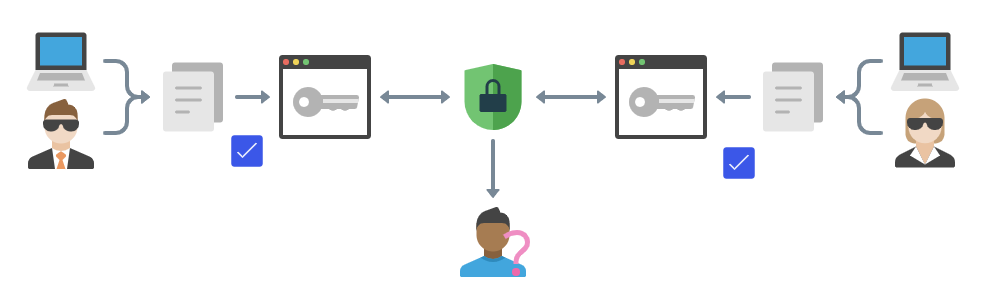
\includegraphics[width=\linewidth]{Private-Public_Key.png}
  	\text{Fonte: Desenvolvido pelo autor com assets disponíveis em \cite{WHIM}}\\	
  \end{figure}

\subsection{A tecnologia blockchain}\index{Blockchain}

O blockchain surgiu como uma forma de organizar de forma segura as transações com criptomoedas de forma imutável. Imagine o Blockchain como um grande de banco de dados distribuído, um livro-caixa de registros de transações, onde aquilo que é registrado não pode ser alterado sendo então uma forma segura de compartilhamento entre redes e usuários, sendo gerenciados de forma autônoma\footnote{De tal forma que não há um mestre administrador, todos aqueles que utilizam do sistema são administradores.}. Se tratando de educação financeira, a tecnologia de blockchain tem grande potencial de aumentar a literacia e o interesse geral da população sobre os criptoativos. 

\section{Os criptoativos}

\subsection{Conceito}
\index{Moedas virtuais}
Os criptoativos são moedas virtuais. Moedas virtuais são um valor monetário representado unicamente por forma eletrônica. Assim como o dinheiro digital, estes também são gerenciados, armazenados ou transacionados de forma eletrônica por meio de sistemas computadorizados, especialmente pela Internet, porém estes não possuem uma contrapartida física. Por exemplo, a quantidade de reais em sua conta bancária online hoje são dinheiro digital porque eles assumem uma forma física quando você os saca em um ATM, diferente do dinheiro virtual. Estes são emitidos por grupos de desenvolvedores ou empresas privadas e, em sua grandíssima maioria, não são regulamentadas. Chamamos estas de descentralizadas.	
 
 \subsection{Concepção}
  A razão pelo qual este capítulo iniciou falando sobre criptografia é porque as criptomoedas utilizam da criptografia para sua segurança.
 O Bitcoin foi a primeira implementação do conceito hoje conhecido como criptomoeda, cujo foi descrito inicialmente em 1998 por Wei Dai na lista de mala direta de discussão cypherpunks\footnote{Um cypherpunk é qualquer indivíduo que defende o uso generalizado de criptografia  e tecnologias que aumentam a privacidade no objetivo de se obterem mudanças sociais e políticas. Sua comunicação original deu-se por meio da lista de mala direta Cypherpunks\index{Cypherpunks}, que uniam grupos informais que almejavam privacidade e segurança por meio do uso intenso de criptografia.}, sugerindo a ideia de uma nova forma de dinheiro que usa criptografia para controlar sua criação e transações, ao invés de um autoridade central. A primeira especificação e prova de \index{Prova de trabalho} trabalho(PoW)\footnote{Aqui estou fazendo uma tradução livre. Segundo \cite{INVPD1} uma ``proof of work'' ou uma prova de trabalho é uma evidência de que um certo poder computacional foi utilizado para resolver um desafio matemático arbitrário em um sistema controlado. As provas de trabalho são amplamente utilizadas hoje em dia na mineração de criptomoedas, para validar transações e minerar novos tokens.}\footnote{Segundo \cite{NAKAMOTO} , O protocolo PoW envolve escanear um valor utilizando a função hash, como a função SHA-256, onde o hash \index{Hash}começa com n bits de valor 0 (Veremos rapidamente sobre esta notação no capítulo de aplicação de atividade). O trabalho médio requerido é exponencial ao número de bits 0 e podem ser verificados utilizando um único hash.} do Bitcoin foi publicada em 2009 em uma lista de discussão de criptografia por Satoshi Nakamoto. Satoshi deixou o projeto no final de 2010 sem revelar muito sobre si mesmo. A comunidade cresceu exponencialmente com muitos desenvolvedores trabalhando em Bitcoin. \cite{BTCPROJ}

\subsection{Receptividade no mundo e na sociedade brasileira}

\subsubsection{No mundo}
Como já foi citado anteriormente, por enquanto a descentralização continua sendo uma atribuição  frequente aos criptoativos devido ao seu curto tempo de existência, sendo uma vantagem segundo os investidores devido a privacidade e a fuga de burocracias e taxas possibilitadas pela independência de intermediários. Segundo \cite{NP}, os bancos centrais de diferentes países têm intensificado críticas, argumentando que o dinheiro digital têm poucos mecanismos para resgate e que “operam contra o bem público”. 

\begin{citacao}\index{Legalidade}
	Apesar disso, as criptomoedas não são ilegais pois atuam em um vácuo de legislação sobre o tema a nível mundial. A tecnologia opera como acordo mútuo entre duas partes, que concordam que a moeda tem valor e que podem estar em qualquer lugar do mundo. \cite{NP}
	\end{citacao}   

\subsubsection{No Brasil} 
Até o presente momento as criptomoedas ainda não são regulamentadas, mas já há uma maior aceitação por parte das autoridades\footnote{Recentemente, um projeto de lei (\textbf{PL}) uma proposta pela tentativa de regulamentação das criptomoedas foi aprovada na câmara dos deputados. Segundo a reportagem veiculada em \cite{JORNALBR}, o objetivo da lei é a prevenção da lavagem de dinheiro e o combate às fraudes. Até o fim da edição deste documento, o PL ainda segue para averiguação do senado federal. } e do banco central brasileiro e o governo quando se tratam deste tema se compararmos com algumas dissertações sobre este tema de anos anteriores. \index{Criptomoeda}\index{Regulamentação}

Segundo o presidente Gilson Finkelsztain da bolsa de valores brasileira, a \textit{B3}, ``É natural que façamos expansão para o mundo não regulado das criptos'' e que segundo ele, já há alguns planos que a \textit{B3} pretende oferecer infraestrutura para negociação de criptoativos. ``Não é uma bolsa de cripto, mas entrar nesse mercado para oferecer serviços para quem negocia cripto'', explicou. \cite{B3} \index{Bolsa de valores}

\index{Blockchain}
E seguindo para uma tendência na tecnologia de blockchain, segundo \cite{UOL} o banco central brasileiro já tem planos de ampliar as formas de pagamento no país criando sua própria CDBC\footnote{CDBC é uma sigla que vem do inglês que significa Central Bank Digital Currency, ou moeda digital de banco central, que como o próprio nome cita, são moedas centralizadas controladas por uma única entidade, um banco central.}, entitulada real digital, uma moeda virtual cujas expectativas são o aumento da inovação, criando soluções que não eram viáveis com o dinheiro em papel ou então barateando soluções que já estão em regime de produção. Ainda segundo a reportagem, 

\subsection{Proposta de modelo de pesquisa (com questionário)} \index{Avaliação}
Ao desenrolar do desenvolvimento deste instrumento, o autor depara-se com a notícia veiculada em \cite{DINO}, que  afirma que 99\% dos brasileiros não conseguem passar em uma avaliação de conhecimento básico de criptomoedas. A avaliação permitia que pessoas de todo o mundo pudessem testar seu nível de compreensão sobre criptomoeda e identificar onde elas precisam aprimorar o conhecimento.

\begin{citacao}
	Como mostra a taxa de aprovação do questionário, existe uma lacuna significativa do conhecimento no Brasil, México e EUA. Nos EUA, quatro em cada 10 entrevistados não conseguiram responder a mais da metade das perguntas, escolhendo 'não sei'. No entanto, os americanos tiveram um desempenho melhor do que os brasileiros, com três em cada 10 respondendo corretamente a cerca de um terço das perguntas do questionário. No geral, os países têm taxas de adoção semelhantes (14\% no México, 15\% no Brasil, 17\% nos EUA). \cite{DINO}
	\end{citacao} 

Um dos objetivos gerais \footnote{Visto na seção \ref{objetivos}} deste instrumento é disseminar criptoliteracia que é o conhecimento sobre criptomoedas argumentando sobre suas funções e características para que na esperança de em algum momento no futuro estes sejam acessíveis e de fácil compreensão, independentemente da renda, status educacional ou sexo, com isso propõe-se uma pequena pesquisa para averiguar em uma escala, de forma local e ainda menor do que adotada pela reportagem,  sobre o tema\footnote{Antes de prosseguir para a subseção (\ref{pesquisa_quest}), recomenda-se ir até a seção do apêndice(\ref{appendix}), onde a pesquisa está disponível para consulta}.  

\subsubsection{Resolução do teste rápido apresentado} \index{Questionário}\label{pesquisa_quest}

As cinco questões aqui apresentadas foram adaptadas da pesquisa oficial disponível na reportagem para que haja uma melhor contextualização dos leitores. Não obstante, se o participante responde qualquer opção diferente de ``Nunca ouvi falar'' na questão sobre sua familiaridade com os criptoativos, este então segue o fluxo usual para a seção do teste. Seguem então suas respostas:



\rule{\linewidth}{0.5mm}
Pergunta: Quais destas frases melhor descreve um criptoativo?
\begin{itemize}
	\item \fbox{Dinheiro que pode ser armazenado fisicamente ou eletronicamente}\index{Criptoativo}
	
	Sim, apesar de existirem carteiras físicas para armazenamento de criptoativos, esta não é a melhor alternativa.
	
	\item \fbox{Dinheiro em papel que só podem ser usados para transações físicas}
	
	Esta alternativa é incorreta pois os criptoativos não são feitos de papel-moeda. 
	
	\item \fbox{Uma moeda digital ou virtual protegida por criptografia}
	
	Correto! Esta alternativa é a melhor opção pois cita a criptografia, base fundamental dos criptoativos.
	
	\item \fbox{Moeda que só pode ser usada para remessas internacionais}
	
	Esta alternativa é incorreta pois apesar das criptomoedas serem uma excelente opção para remessas internacionais, estes não ficam limitadas somente nesta função. 
		
	\item \fbox{Eu não sei}\\ Opção que indica que o participante prefere não arriscar uma resposta.

\end{itemize}

\rule{\linewidth}{0.5mm}

Pergunta: Quais destes você acredita que não seja uma criptomoeda?

\begin{itemize}
	\item \fbox{Ethereum}\index{Ethereum}
	
	Opção incorreta. O Ethereum (ETH) é uma criptomoeda descentralizada que teve seu lançamento em 2015.
	
	\item \fbox{Litecoin}\index{Litecoin}
	
	Opção incorreta. O Litecoin (LTC) é uma criptomoeda muito semelhante ao bitcoin que teve seu início em 2011.
	
	\item \fbox{Dogecoin} \index{Dogecoin}
	
	 Opção incorreta. O Dogecoin (DOGE) é uma criptomoeda que foi criada com a temática do meme Doge, um cachorro da raça shiba inu. 
	 
	\item \fbox{Metamask}\index{Metamask}
	
	 Opção correta! O metamask é uma carteira digital que permite guardar e transacionar criptomoedas e não uma criptomoeda em si.
	 
	\item \fbox{Stellar Lumens} \index{Stellar Lumens}
	
	Opção incorreta. O Stellar Lumens (XLM) é uma criptomoeda criada em 2014.
	
	\item \fbox{Eu Não sei} 
	
	Opção que indica que o participante prefere não arriscar uma resposta.
\end{itemize}

\rule{\linewidth}{0.5mm}

Pergunta: O que é a mineração de criptomoedas?
\index{Mineração}
\begin{itemize}

	\item \fbox{\begin{minipage}{\linewidth}{
	Uma rede de carteiras físicas e digitais enviando e recebendo ativos digitais entre si,mantendo a segurança do blockchain, é o processo que aumenta a quantidade de moedas em circulação.}\end{minipage}}

 Opção correta! Esta opção é a que melhor define a mineração de criptoativos.
 
	\item \fbox{\begin{minipage}{\linewidth}{Um aplicativo de telefone onde os usuários resolvem ou jogam jogos e recebem criptomoedas como recompensa}\end{minipage}}
	
	Opção incorreta.
	
	\item \fbox{\begin{minipage}{\linewidth}{O processo de mineração de metais preciosos para financiar o desenvolvimento de um projeto de criptografia}\end{minipage}} 
	
	Opção incorreta. O termo ``minerar'' também pode ser usado na extração de minério, mas não tem relação direta com a mineração de criptoativos.
	 
	\item \fbox{Eu não sei}
	
	Opção que indica que o participante prefere não arriscar uma resposta.
	
\end{itemize}

\rule{\linewidth}{0.5mm} \index{Divisibilidade}

Pergunta: Moedas regulamentadas, apoiadas por bancos centrais, tem divisibilidade limitada. Um real, por exemplo, só pode ser dividido em 100 partes de
centavo, cada uma valendo R\$ 0,01. Quantas unidades, ou casas decimais, um bitcoin pode ser dividido?

\begin{itemize}
	\item \fbox{3 casas decimais} 
	
	Opção incorreta. 
	
	\item \fbox{8 casas decimais}  
	
	Opção correta!
	Um bitcoin é divisível em oito casas decimais (100 milionésimos de um bitcoin), e esta menor unidade é denominada de  um Satoshi em homenagem ao seu criador, Satoshi Nakamoto.
	
	\item \fbox{20 casas decimais}
	
	Opção incorreta.  
	
	\item \fbox{Nenhum. Você não pode dividir um bitcoin em um decimal} 
	
	Opção incorreta. 
	 
	\item \fbox{Eu Não sei} 
	
	Opção que indica que o participante prefere não arriscar uma resposta.
	
\end{itemize}

\rule{\linewidth}{0.5mm} \index{Métricas}

  Qual métrica é usada para medir o poder de processamento de uma rede de
  mineração de criptomoedas?

\begin{itemize}

	\item \fbox{CPUs} 
	
	 Opção incorreta. CPUs  são denominados por Central Process Unit, ou Unidade Central de Processamento. São o principal componente de hardware de um computador.
	 
	\item \fbox{Hashrates (h/s)}
	
	 Opção correta!  Hashes por segundo indicam a quantidade de operações computacionais que um sistema ou  rede de mineração é capaz de realizar em um segundo.
	 
	\item \fbox{Megahertz (MHz)}
	
	Opção incorreta.
	
	\item \fbox{Gigahertz (GHz)} 
	
	Opção incorreta.
	
	\item \fbox{Eu Não sei}
	
	Opção que indica que o participante prefere não arriscar uma resposta.
	
\end{itemize}


 
